% !TEX root = ../Thesis.tex
\chapter{Implementation}
\label{c:implementation}

This chapter describes an implementation in correspondence to the concepts proposed and ellaborated in chapter \ref{c:concept}. 
These concepts are applied to Polypheny-DB, a particular polystore system.\\
First the current architecture and all relevant components and modules of this system are described. Afterwards each proposition of the concept is adapted
so it can be implemented within Polypheny-DB to enrich it with freshness-aware data management.
This chapter is separated into several building blocks, where each part is necessary to describe the implementation in accordance with the requirements.
It is abstracted into two main sections. The first addresses the functional requirements (i, iii, iv) and aims to apply the concepts of Lazy Replication with all its
cross-dependencies, while the second part focuses on introducing the notion of freshness itself, hence aiming to provide the requirements (ii, v, vi).
Finally, all building blocks are gathered and put into perspective to describe an entire lifecycle for freshness within Polypheny-DB. 


%%%%%%%%%%%%%%%%%%%%%%%%%%%%%%%%%%%%%%%%%%%%%%%%%%%%%%%%%%%%%%%%%%
%%%%%%%%%%%%%%%%%%%%%%%%%%%%%%%%%%%%%%%%%%%%%%%%%%%%%%%%%%%%%%%%%%
%%%%%%%%%%%%%%%%%%%%%%%%%%%%%%%%%%%%%%%%%%%%%%%%%%%%%%%%%%%%%%%%%%



\section{Polypheny-DB}
\label{sec:architecture}


The implementation is based on the polystore system Polypheny-DB\footnote{https://github.com/polypheny/Polypheny-DB}.
In this chapter we briefly describe and illustrate a simplified version of Polypheny-DBs current architecture.
As well as some fundamenetal components that will be throughout this chapter\\
This extends the foundations laid out in Chapter \ref{c:Foundation} and sets them in context of the existing system model.\\




\emph{Polypheny-DB} is an Open-Source project\footnote{https://polypheny.org/} developed by 
the \textit{Database and Information Systems} (DBIS) group of the University of Basel.
It is a self-adaptive polystore that provides cost- and workload aware access to heterogeneous data\cite{poly2020}.

Compared to other systems like \textit{C-Store}\cite{cstore_2005} or \textit{SAP HANA} \cite{hana_2012}, 
Polypheny-DB does not provide its own set of different storage engines to support 
different workload demands.\\
Instead, it acts as a higher-order DBMS which provides a single-point of entry to 
a variety of possible databases like 
\textit{MongoDB}\footnote{https://www.mongodb.com/}, 
\textit{Neo4j}\footnote{https://neo4j.com/},
\textit{PostgreSQL}\footnote{https://www.postgresql.org/} 
and \textit{MonetDB}\footnote{https://www.monetdb.org/}. 
These can be integrated, attached and managed by Polypheny-DB which will incorporate the underlying 
heterogenous data storage engines with their different data structures. 
It is desigend to abstract applications from the physical execution engine while profiting from 
performance improvements through cross-engine executions. 
\\
For incoming queries Polypheny-DB's routing engine will automatically analyze the query and decide 
which store will provide the best response. The query is then explicitly routed to these data stores. 
This approach can be characterized as a dynamically optimizing data management layer for different workloads.\\
Due to its inherent architecture and the possibility to replicate data across different homogenous as well as heterogeneous stores, it is also able to cluster, specific stores 
on a table entity level, although the underlying stores might not support this natively. 
This leverages Polypheny-DB to a data orchestration platform towards an actual PolyDBMS ~\cite{polypheny2021}. 



\todoMissing{polypheny support multi-model databsaes for relational, document, graph in memroy ...}

%%%%%%%%%%%%%%%%%%%%%%%%%%%%%%%%%%%%%%%%%%%%%%%%%%%%%%%%%%%%%%%%%%

\subsection{Placements}
Placements are considered to be Polyphenys virtual representation of physical entities.
Since Polypheny provides a multi model approach, underlying stores can range from relational to document until graph engines. 
Entities are therefore a genereal definition encompassing tables, collection or graphs, respectiviely of the utilized model.
They act as an abstraction between the polystore layer and the physical representation of an entity. 
Mostly used within the PolyDBMS itself they help to assist the logical routing process of Polypheny-DB.

\todoMissing{remove replication strategy from image}
\begin{figure}[t]
    \centering
    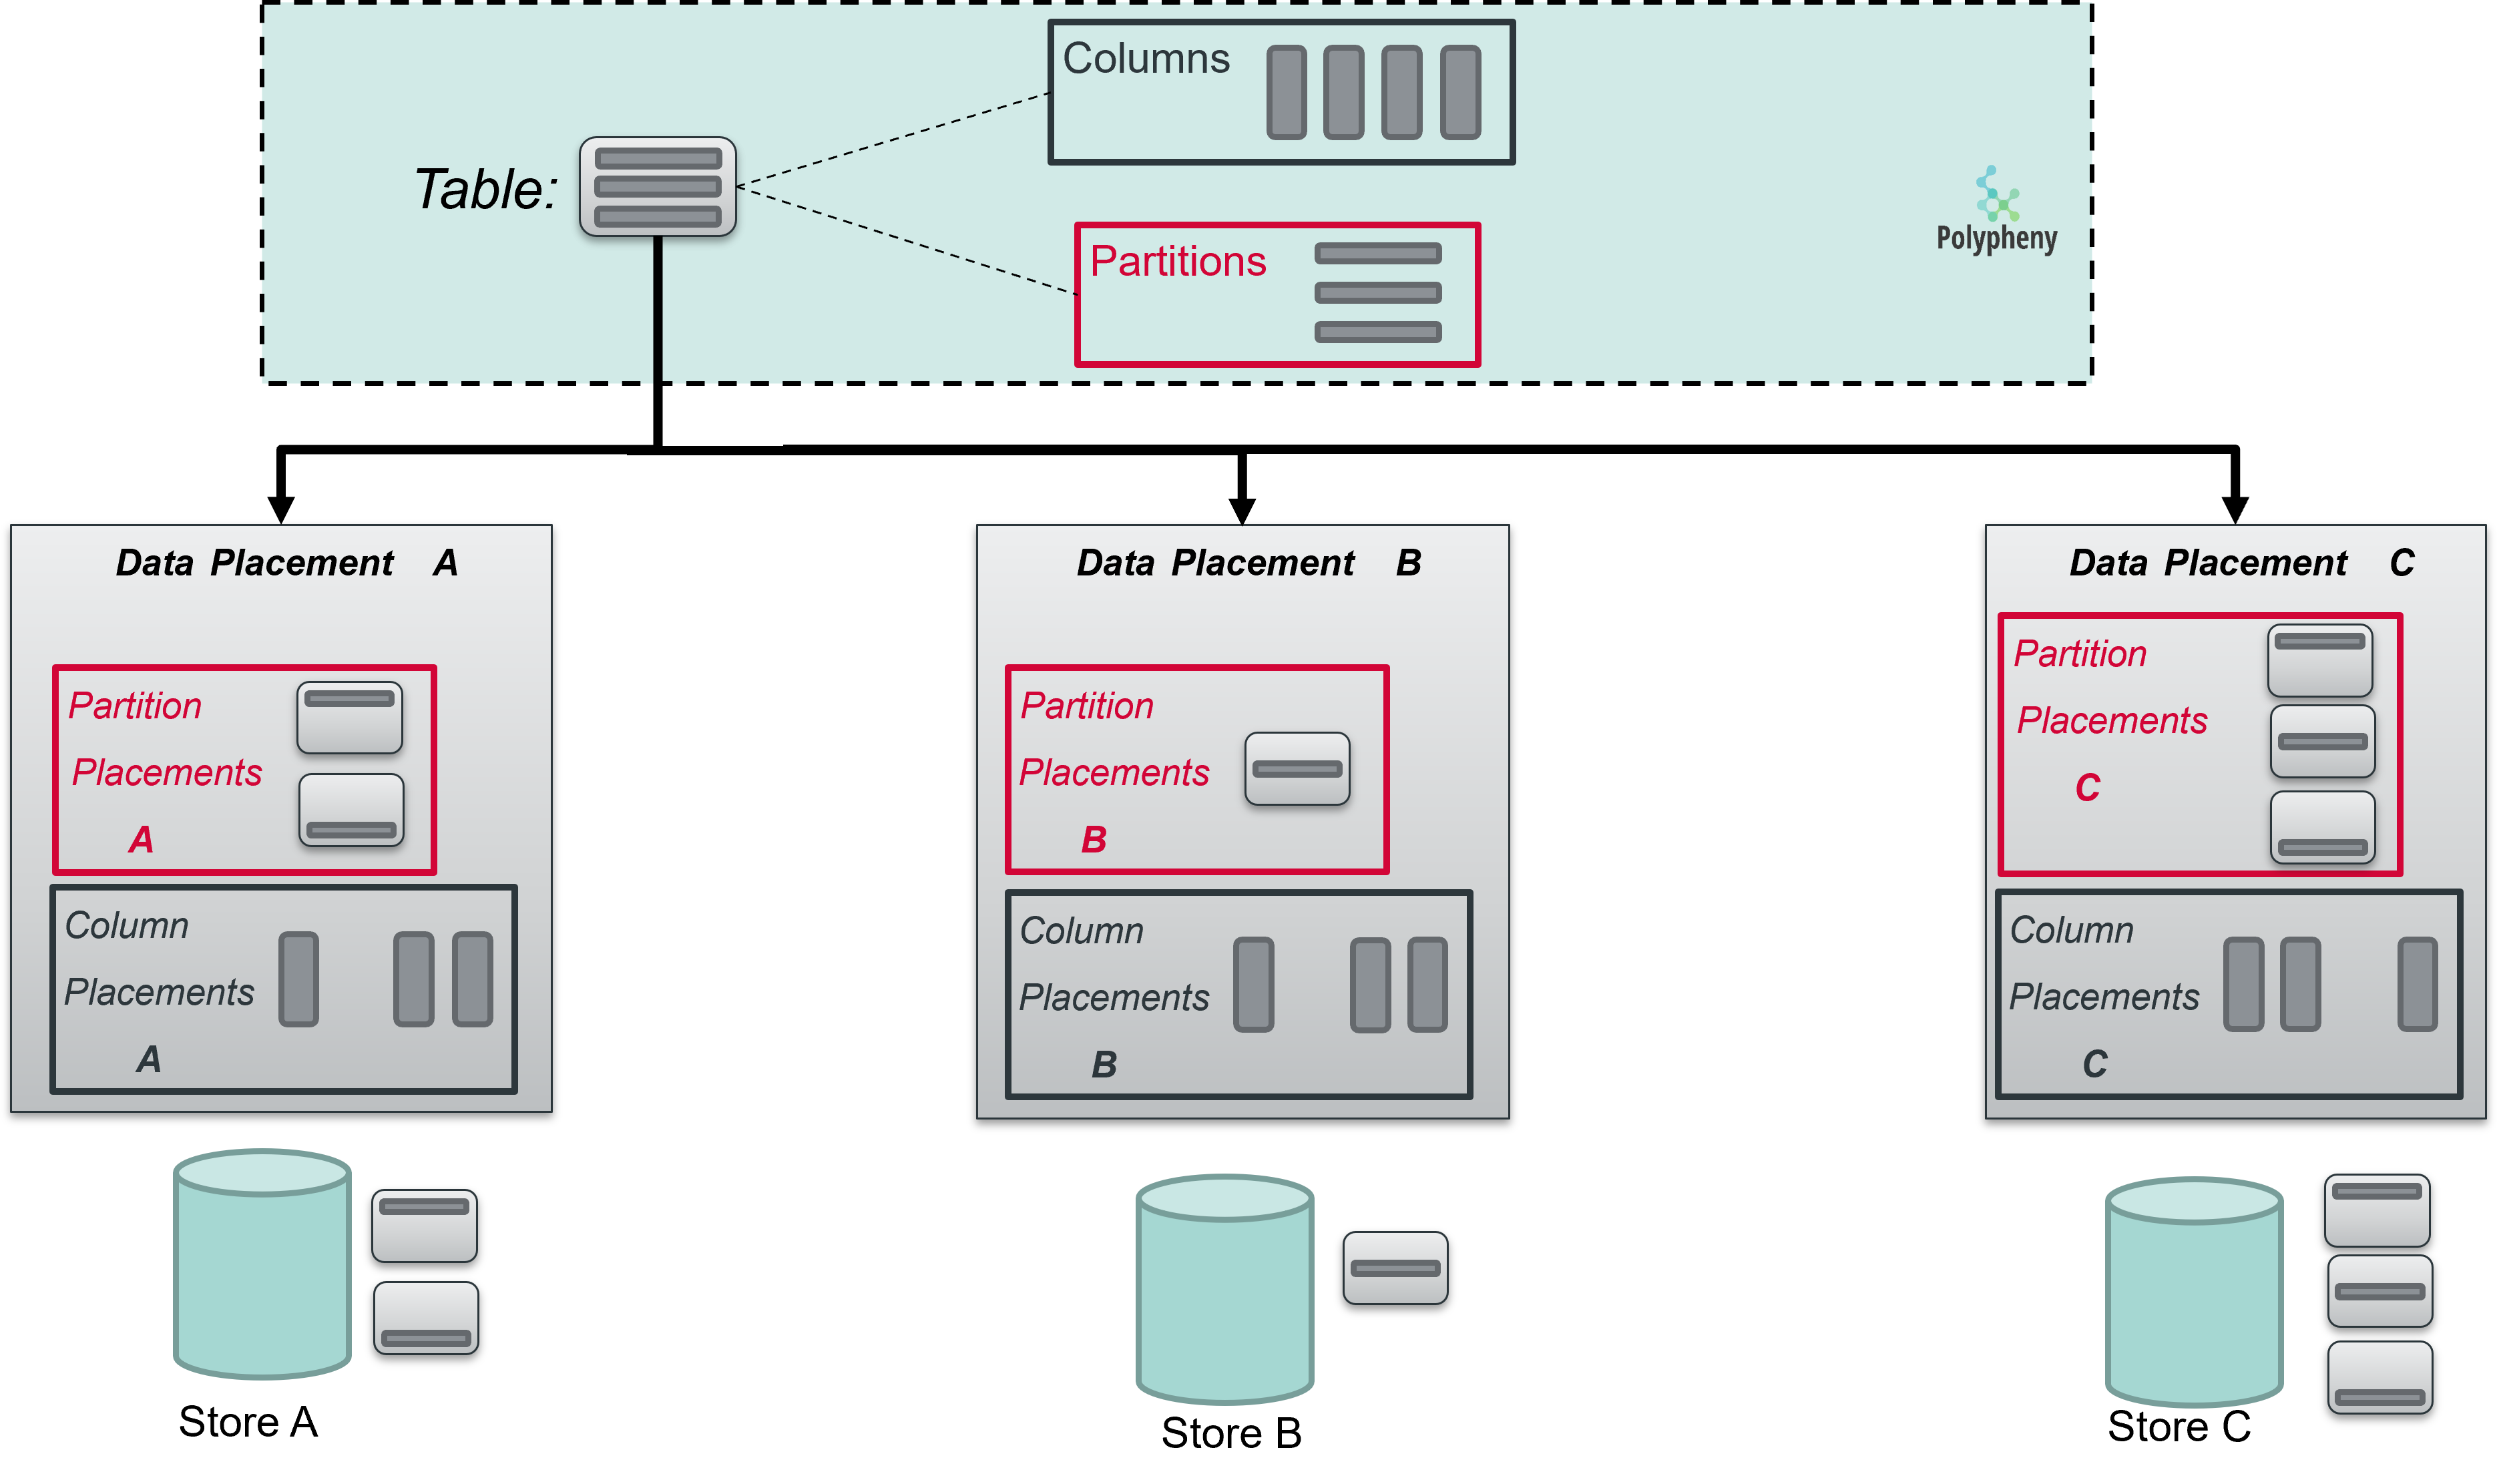
\includegraphics[width=0.7\textwidth]{Figures/data_placement.png}
    \caption{Polypheny-DB's entity representaiton via placements. Mapping a logical entity to the actual physical stores.}
    \label{fig:placements}
\end{figure}

\begin{description}
    \item [Data Placements] A Data Placement is essentially a virtual representation of the physical entity residing on a given store.
    A store in Polypheny is an underlying physical data storage which is attached to Polypheny-DB.
    All attached stores can be used to hold several fragments of data. 
    During routing decisions stores are automatically taken into consideration if they are designated for the associated data.
    
    A Data Placment contains information on available columns ($\rightarrow$ Column Placements), partitions ($\rightarrow$ Partition Placements)
    as well as properties that are unique to this store. These properties are centrally configured per Data Placement but will be passed on to the underlying placements as well.
    
    When an entity is created on Polypheny-DB it is an ordinary structure placed onto one store.
    An entity can therefore contain several Data Placements with different capabilities and properties as depicted in figure \ref{fig:placements}. 
    
    

    \item [Column Placements]
    Are part of the virtual representation of a physical entity. They are essentially needed to fulfill the intended flexibility of Polypheny-DB. 
    Column Placements are considered to be instances of a column placed on a specific store.
    These placements are the result of the extended vertical partitoning of an entity.


    As already discussed in \ref{sec:part}, vertical partitioning refers to the logical 
    separation of the data structure by columns to obtain logically connected objects throughout 
    the database. Polypheny-DB extends this functionality to vertically partition tables
    column wise, which allows a table itself to be split further into a disjoint 
    set of columns.
    Column Placements are instances of a column placed on a specific store.
    They are considered unique per column on a cluster.
    Since an entity consists of one to \textit{n}-columns.
    In the context of vertical partitioning a subset of these \textit{n}-columns can now 
    be placed onto another store, which will consequently be part of a \textit{Data Placement}.
    This can either be done by evenly distributing the columns onto these stores 
    or by simply replicating the subset to a second store.
    This functionality enables Polypheny-DB to adapt the data structure to continuously 
    varying use cases.\\

   

    \item [Partition Placements] Although, part of the Data Placement as well, a Partition Placement is considered to be the actual virtual representation of a physical entity.
    It essentially represents and links to the physical entity stored on an underlying engine. Partition Placements are the results of applying a partition function to an entity,
    to horizontally partition the entity into a distinct set of rows. The resulting partition placements can then be placed freely on existing stores to distribute or replicate data.\\
    Due to the partition function \emph{NONE} every entity inside Polypheny-DB is considered to be partitioned. Hence consisting only of one partition.
    Additioanlly, Polypheny suppports the most common partition algorithms like \emph{HASH}, \emph{RANGE}- and \emph{LIST}-Partitioning. 
    It allows to selectiviely query independent placements respectiviely distinct underlying physical stores, to distribute incoming workload evenly within the cluster.
    Together with Column Placements they provide great flexbility to adapt and customize any system, to fit various requiremnts.
    
\end{description}



%%%%%%%%%%%%%%%%%%%%%%%%%%%%%%%%%%%%%%%%%%%%%%%%%%%%%%%%%%%%%%%%%%


\subsection{Query Routing}
\label{sec:routing}

The query routing is an essential part of any polystore system and is crucial for Polypheny-DB's processing capabilities.
The routing process can be briefly described as an abstraction layer that will locate and consequently provide the best combination of suitable Data Placements to fulfil a given request 
or to provide a given result. \\
The Routing Process can roughly be distinguished in four phases. A \emph{resolving phase} which identifies individual building blocks such as partitions which are necessary 
for the query execution. The second phase is referred to as \emph{parametrization} and is used to transform the statement into cachable object to simplify further routing steps.
Followed by the time-consuming \emph{planning phase} which generates and proposes possible execution plans to determine on which store and placement combinations a query should be executed.
This is finalized by the \emph{selection phase} which is build on top of the previously generated candidate plans and will effectiviely pick the best suitable plan for a 
given execution. Since especially the time consuming generation of possible plans can get quite large for highly distributed entitites, allowing for a large set of 
possible combinaitons, this phase can be cached.
This enables pre-delivering already geenrated plans for similar queries to be used by the last phase to save processing time and reduce overhead ~\cite{vogt_dis_2022}.\\


Since every query has to go through the abstraction layer to guarantee correctness 
and consistency, Polypheny-DB can consult the systems internal \textit{Catalog} to retrieve the
location of all relevant data. 
If the requested data indeed happens to be distributed on several stores. The central routing engine will join all relevant and distinct 
placements to construct the result set. Hence, the query is always routed to stores which hold relevant data.\\


Given Polyphenys current architecture all incoming queries have to be delivered through this central polylayer, acting as a central instance.
Since we assume that there is no direct interaction with the underlying systems there is no immediate risk of inconsistencies. 
This allows the utilization of SS2PL to handle concurrency control only within Polypheny-DB for correct isolation treatment.
While this provides a serializable execution of each operation by applying suitable locking capabilities, it impacts the availability respectiviely the latency of the entire system.
Since Polypheny-DB has to ensure global consistency, it needs to apply a lock on the entire entity that is accessed. 
For highly distributed entities, Polypheny-DB has to ensure that every write-operation is applied equally on all stores.
This blocks further processing until the operation has been persisted and ultiamtely commited by all underlying stores,
which introduces a bottleneck for this layer, that is inherently dependend on the slowest performing store.






%%%%%%%%%%%%%%%%%%%%%%%%%%%%%%%%%%%%%%%%%%%%%%%%%%%%%%%%%%%%%%%%%%
%%%%%%%%%%%%%%%%%%%%%%%%%%%%%%%%%%%%%%%%%%%%%%%%%%%%%%%%%%%%%%%%%%
%%%%%%%%%%%%%%%%%%%%%%%%%%%%%%%%%%%%%%%%%%%%%%%%%%%%%%%%%%%%%%%%%%


\todoMissing{Maybe rename?}
\section{Lazy Replication}
\label{sec:lazy_replication}

This section discusses all implementations along with the introduced components and services to establish 
multi versioning and the possibility to refresh specific replicas. This serves as a foundation in order to use those distinct versions
to be used within query retrieval. Which again shall help to reduce the overall latency of the system by allowing mixed workload to exist in parallel.

\todoMissing{In correspondence to the section \ref{sec:propagation} update propagtion in concept we focussed on implementing the CDC approach ($\rightarrow$ \ref{sec:algo}) 
as well as the on-demand approach using primary Snapshot Copy ($\rightarrow$ \ref{sec:manual_refresh}))}


\subsection{Placement Versioning}

As we have established in section \ref{sec:data_replicas}, the existence of multiple data replicas are fundamental in distributed systems to even provide the 
possibility of a trade-off between latency and consistency. These versions essentially allow load balancing requests among all suitable replicas to effectively 
use the entirety of the system. This does not only enable one to distribute the load evenly across the landscape, hence increasing the availability.
But also defines how many of these replicas need to utilized jointly to enforce the desired consistency constraints.\\

As the name might suggest, a multi-version database would be ideal and the obvious choice for such an approach.
These databases will automatically generate a new version per data object for each modification. 
Due to their properties we would immediately have the information on the validity-interval of the version, its update time as well as predecessor and successor versions.
This would directly allow us to utilize these versions on freshness-related queries. 
However, as stated in \ref{sec:concurrency_control} multi-version databases automatically tend to have larger data footprints, due to persisting  
redundant and even obsolete data.
However, polystore systems already suffer from a larger data volume, given the redundant data storage across severall stores.
Furthermore, this would also consequently imply the utilization of MVCC.
But aforementioned, Polypheny-DB currently only supports SS2PL for its concurrency control.
Since we require to have equally converging states for our outdated versions \textit{(iv)}, we need a serializable execution that can be applied to 
the underlying stores as well.
Although, MVCC reduces common blocking scenarios and allows write- and read-operations to be executed in parallel, 
it cannot reliably produce a serializable execution order of all operations among all participating stores.
That is why we remain with SS2PL and refrain from using the automatic versioning provided by a multi-version database.\\

However, as already mentioned in chapter \ref{c:concept}, multiple versions are automatically created when using a lazy update propagation among the participating nodes. 
This will directly loosen the constraints, imposed on replicas to update. 
The update in these cases will then only be targeted towards the primary replicas, drastically reducing the reponse time of a write-operation,
but lowering the consistency at the same time.  \todoMissing{Besserer Übergang}
Furthermore, to provide freshness-awareness as well, we do not only require several versions for updates to be applied quicker,
but also be able to actually utilize these versions to efficiently operate on the entire system.
These versions therefore also allow us to compare and find suitable candidates in freshness related queries.\\

Fortunately, polystore systems and especially Polypheny-DB is inherently distributed, automatically providing potentially multiple replicas.
Although they might be distributed or replicated, resulting in redundant data storage, Polypheny-DB allows to create multiple data placements for an individual entity.
The introduced data placements described above can therefore be considered as an individual replica or version for a corresponding data item as referred to in the concept.
Therefore to enable Polypheny-DB to retain different levels of freshness we need to allow our routing process
to only target a subset of all placements for primary update transactions. The remaining placements will therefore autoamtically become outdated. 

However, since partition placements logically refer to the physical entities that actually persist the data and 
read-only queries typically benefit directly from data partitioning (see \ref{sec:part}), Polypheny-DBs partition placements 
are suitable candidates to base our freshness awareness on.




%%%%%%%%%%%%%%%%%%%%%%%%%%%%%%%%%%%%%%%%%%%

\subsection{Replication Strategy}
\label{sec:strategy}

In order to reduce the update time per write-operation and increase the performance
of OLTP workload, we need to enable Polypheny-DB to identify placements that need to receive updates immediately. 

To allow the routing process to differentiate between such placements,
we need the possibility to label data placments on how they are going to receive updates. This is defined as the \emph{Replication Strategy} $\Gamma \in \{EAGER,LAZY\}$.
\emph{EAGER} means that DML operations are applied at once, while \emph{LAZY}
allows data manipulation to be deferred, resulting in outdated data.\\


Although, we defined that we will base the freshness evaluation on partition placements, we implemented the strategy per data placement. 
As introduced in the beginning of this chapter, partition placements inherit their information from its corresponding data placement.
Although they receive there updates independently their properties are defined within the parent placement. 
Therefore, it is sufficient to configure the data placement to achieve an intended state of the subordinate partition placements.
Such that a partition on a given store can either be updated enitrely eagerly or lazily. 


%Since the locking within Polypheny-DB is done logically within the polystore layer and locks the entire table.
Since we want to establish the freshness comparison based on each individual partition placement, the locking mechanism
has been adapted to allow locking on partition level rather than on a table-level. 
This allows for a much finer level of detail and increases the degree of parallelism. 

Can be used to selectively define which data placement shall be updated lazily.
The replication strategy can therfore be directly defined as:
\begin{lstlisting}[language=sql, caption={SQL Stateemnt Syntax to modify the designated Replication Strategy for a Data Placement},label={lst:strategy}]
ALTER TABLE tableName MODIFY PLACEMENT ON STORE storeName 
                                       WITH REPLICATION ( LAZY | EAGER );
\end{lstlisting}

This replication strategy is added as part of the newly introduced data placement properties. Since Data Placements inherently carry the information, what column and partitions reside
on a given store, they were extended to now also hold information on data placement specific properties.

When a placement is created without any replication strategy, it will automatically be labeled to receive updates eagerly.\\
This allows us to flexibly define the strategy per data placement, considering all necessary constraints to ensure the conssitency and integrity of the data (see \ref{sec:constraints}).


%%%%%%%%%%%%%%%%%%%%%%%%%%%%%%%%%%%%%%%%%%%


\subsection{Replication State}
\label{sec:states}

Since the replication strategy is bound to an individual data placement we still need the possibility to 
define how the actual partition placements, that hold the data, will behave in certain scenarios and will consequently be processed.
We therefore introduce the \emph{Replication State} per partition placement.\\

This replication state is logically bound, and directly influenced by the replication strategy defined within a data placement
and can be differentiated into three states that define the intended state of a given partition placement. 
\begin{description}
    \item [UPTODATE] Is automatically set within a partition placement, when the parent placement is configured to receive updates eagerly.
    This cannot be changed by any user. It does also not refer to the current state of any data object, meaning that an lazily updated placement can become up-to-date overtime.
    Allthough this is possible in terms of the received update, it is not respresented using these states. They rather impact the behaviour and handling during processing.
    
    \item [REFRESHABLE] Initially this is configured when the corresponding data placement receives updates lazily. This allows the partition placement to actively receive 
    individual updates by a replication algorithm. A refreshable state can be automatically and manually transformed into an \emph{INFINITELY OUTDATED} state.

    \item [INFINITELY-OUTDATED] This state is specifically marked, to stay outdated and not receive any updates by suspending all distribution towards those stores.
    This can either be done manually, because a user may want to
    retain an item with a given version, hence surpressing the automatic update replication on this node. Additionally this can be set autoamtically by the system, 
    if either the entire store or the system is not available anymore. This can be caused due to an unexpected outage or simply because the replication algorithm has 
    numerously failed to apply updates, indicating an error. Given certain prerequisites it can be manually transformed back into an \emph{REFRESHABLE} state.

\end{description}

The distinction between these cases is necessary, to allow treating partition placements on a given store differentely. 
Otherwise if one partition placement would be automatically labeled as \emph{INFINITELY OUTDATED} the entire data placement could not be refreshed anymore.
Therefore they are handled and considered independently.

Although, this state is required for internal processing of individual partition placements, the manual specifcation of this state is still 
targeted to an entire data placement (\ref{lst:state}).
Since the internal partitioning should be rather user agnostic one should only be able to specifiy this per data placement. 
As with the replication strategy, the changes are then propagated downwards to all linked partiton placements.\\

However they cannot be set freely and have to follow certain constraints (see \ref{sec:constraints}).
Although Placements containing REFRESHABLE can be set to INFINITELY OUTDAZED and vice versa, the state UPTODATE can only be influenced by the replication strategy.
Trying to change this manually will result in an error since it is controlled by the system.

\begin{lstlisting}[language=sql, caption={SQL Statement Syntax to change the designated Replication State of data placement.},label={lst:state}]
ALTER TABLE tableName MODIFY PLACEMENT ON STORE storeName 
                                       WITH STATE ( REFRESHABLE | OUTDATED );
\end{lstlisting}

Furthermore since each Partition Placement is enriched with the most recent update information to support various freshness metrics,
we propose to define the outdatedness on the state of a specific partition placement.
Although the entire data placement, could be labeled as outdated or rather receive updates lazily, some of 
these partitions could already be up-to-date again, while others still remain outdated.


%%%%%%%%%%%%%%%%%%%%%%%%%%%%%%%%%%%%%%%%%%%

\subsection{Change Data Capture}
\label{sec:cdc_impl}

Influenced by the replication strategies, the routing process is now capable of differentiating between placements needed to be updated immediately or asynchronously. 
When processing a DML-operation, the router can identify for a given entitiy if it contains at least one placement that is updated lazily.
If this is true it will capture all executed changes within a \emph{Change Data Object} to be later applied on these placements. 
Disregarding the operation type $\in \{INSERT,UPDATE,DELETE\}$, it contains information on all logical partitions that have been involved, 
the executed operation, as well as the current statement and transaction id. For \emph{DELETE} and \emph{UPDATE} operations it also stores additional information on possible filter 
conditions. Each statement within a transaction can have at most one of these objects and refers to one operation to be executed.\\

After creation this object will be added along its statement id to a preliminary \emph{capture-queue} within the \emph{Change Data Collector}. 
As visualized in \ref{fig:hashtable} this capture-queue is represented as a hashtable for 
faster retrieval, and maps a transaction to a list of statements that require change data capture. 
These statements are stored with respect to their execution order within the parent transaction.
Each statement inside this structure is attached to its respective \emph{Change Data Object}.\\

\begin{figure}[t]
    \centering
    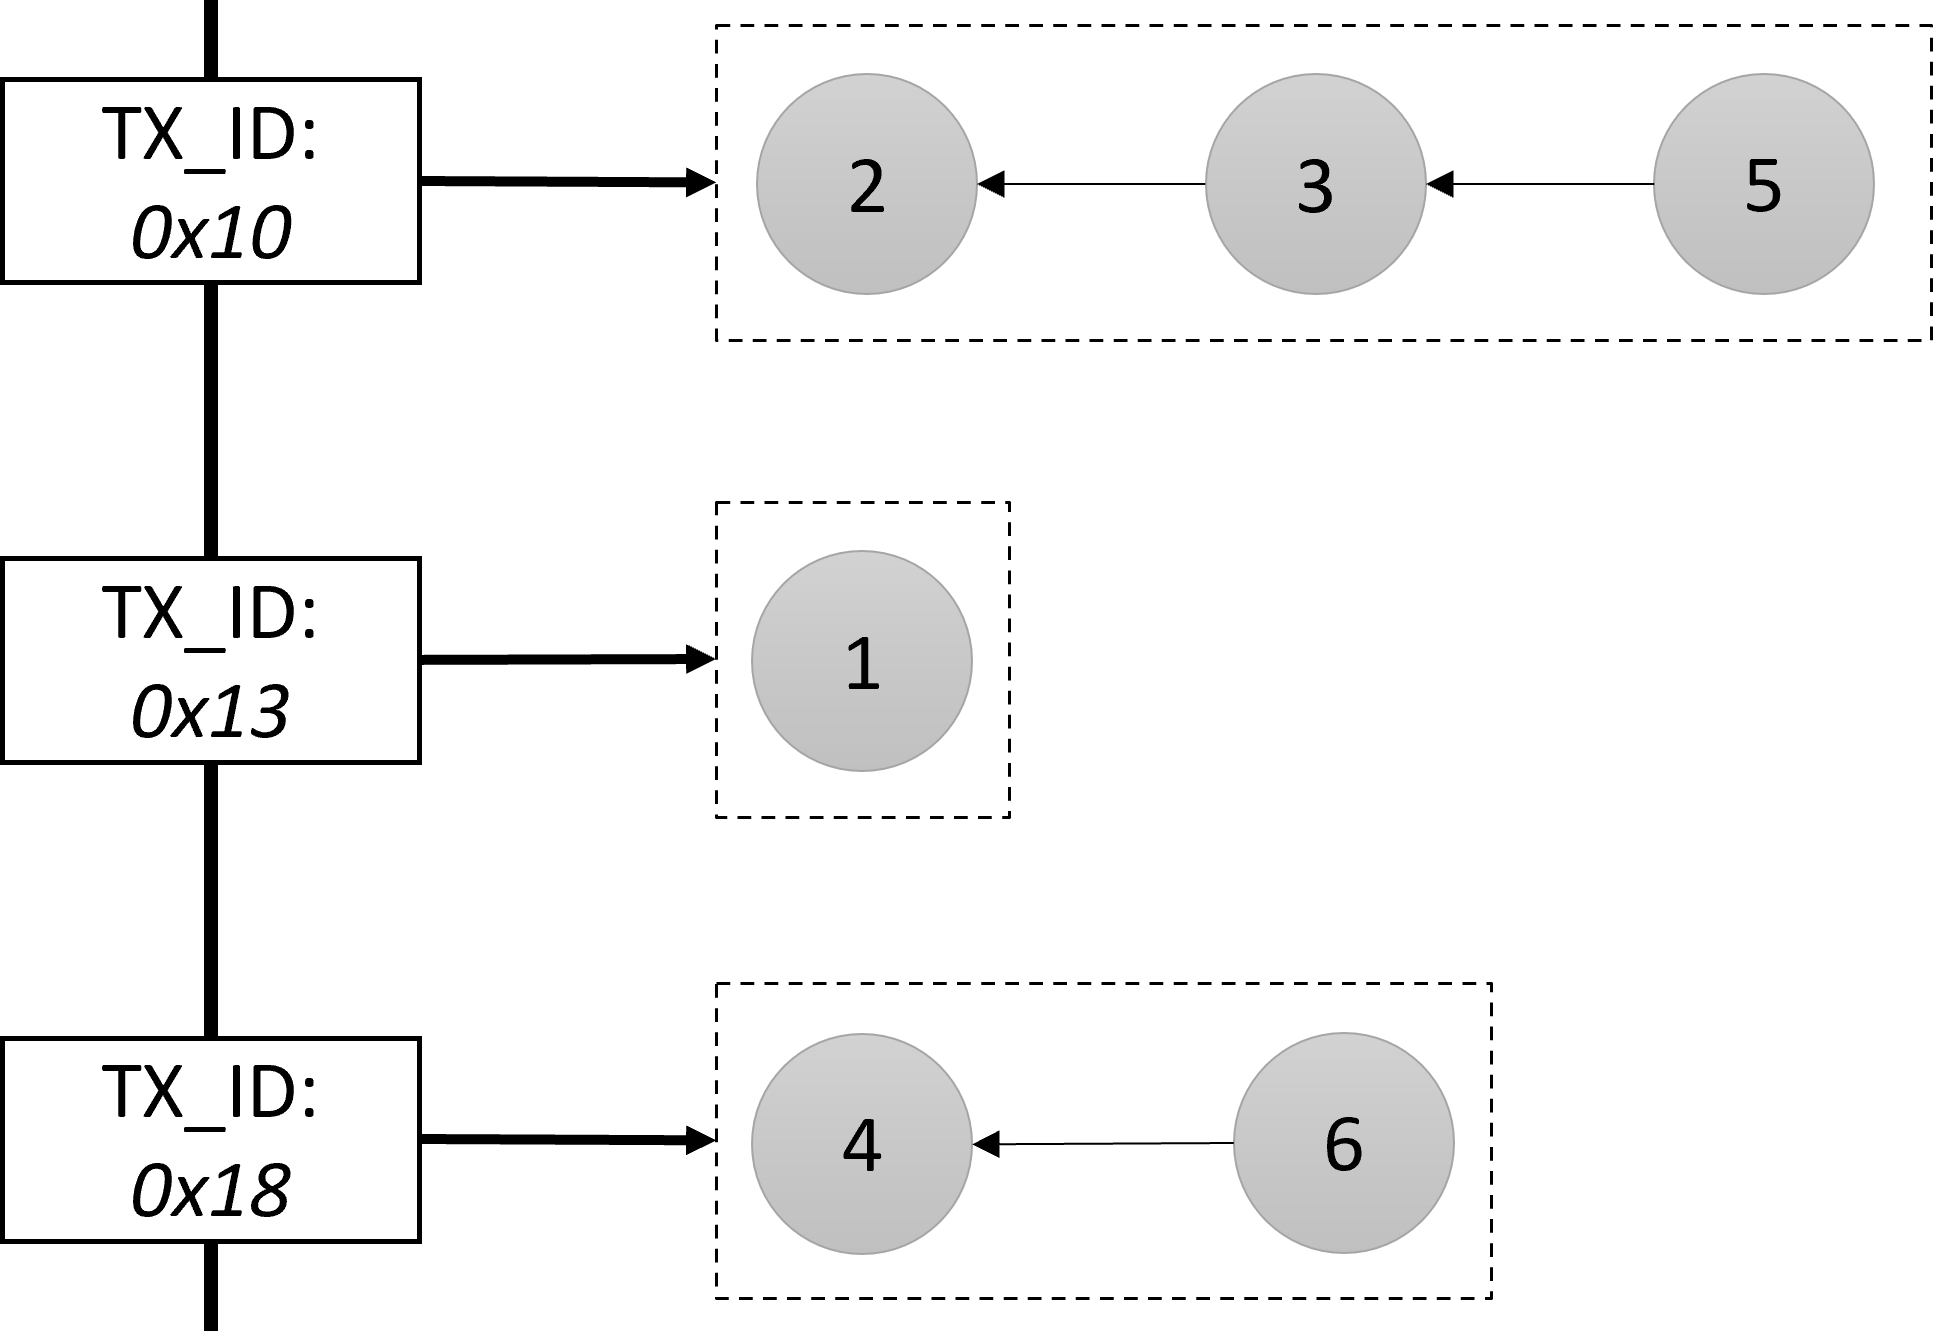
\includegraphics[width=0.5\textwidth]{Figures/hashtable.png}
    \caption{Capture Queue, containing pending transactions as well as an ordered list of executed statements containing the captured data.}
    \label{fig:hashtable}
\end{figure}

To be able to apply operations directly to the outdated replicas, they need to be converted into basic operations that can be applied to a prepared statement.
Therefore they are captured before they are executed but after they have been evaluated.\\
Since not all stores provide the same functional capabilities, we can leverage the polystore-layer to pre-compute certain calls before applying them to the underlying stores.
Typical functions that are not uniformly provided are e.g.: \emph{CURRENT\_TIME} or \emph{TIME\_NOW}. This allows storing the actual values that are executed on the store,
hence saving execution time during update propagation.
During runtime of any given statement the actual evaluated data values are then injected into the object stored within the capture-queue.\\
The benefit of this structure is that as soon as the transaction commits, the \emph{Change Data Collector} is notified, streaming all objects in correct execution order
into the \emph{Replication Engine}, where they will be transformed into individual \emph{Replication Objects} and finally queued to be propagated onto outdated placements. 
Since the registration is done during the commit, we are sure that any pending changes will be available for distribution once the transaction has been commited.



%%%%%%%%%%%%%%%%%%%%%%%%%%%%%%%%%%%%%%%%%%%

\subsection{Lazy Replication Engine}
\label{sec:lazy:_engine}

A \emph{Replication Engine}, contains the core functionality that transforms capture objects into distinct replication objects and 
pipes them to specific execution engines.
The \emph{Lazy Replication Engine} is a specific implementation of the general replication engine and enhances it with several additional capabilities targeting
the lazy replication strategy. This engine essentially provides the CDC approach proposed in section \ref{sec:refresh_operations} and is influenced by the 
change data capture service of section \ref{sec:cdc_impl}, to apply changes operation-wise to designated targets.\\

During commit time of a transaction, all corresponding \emph{Change Data Objects} will be first transformed into distinct \emph{Replication Objects}. Other than
the generic change objects these are restructured and specifically tailored to specific operations and designated targets. During transformation the engine retrieves all 
relevant placements that are currently defined to receive updates lazily. Then for each of these target placements an individual replication object is generated, allowing to 
replicate changes independently from each other. These transformed objects are then added to a \emph{Global Replication Queue} which concludes the change data registration process.\\


The engine itself is decomposed into the following services that jointly allow an asynchronous execution of modifications within Polypheny-DB. 

\begin{description}

    \item[Replication Data Object] This object contains all information, necessary to re-create a statement which is equivalent to the orginal one,
    that has already been executed on the primary placements. 
    Therefore it keeps information on the orginal transaction, its commit time as well as the operation type and the data to be delivered. 
    This is further enriched with a list of all target partition placements that shall receive this modification. The list of targets is generated
    at the time the initial update transaction has been committed and changes have been queued. In order to avoid storing data redundantly, this data object 
    is centrally stored and only referenced by depending replication objects, disregarding the number of placements that shall receive a given DML-operation.
    This data is kept as long as there are replication objects depending on it for executing their replication.


    \item[Global Replication Queue] 
    
    \begin{figure}[t]
        \centering
        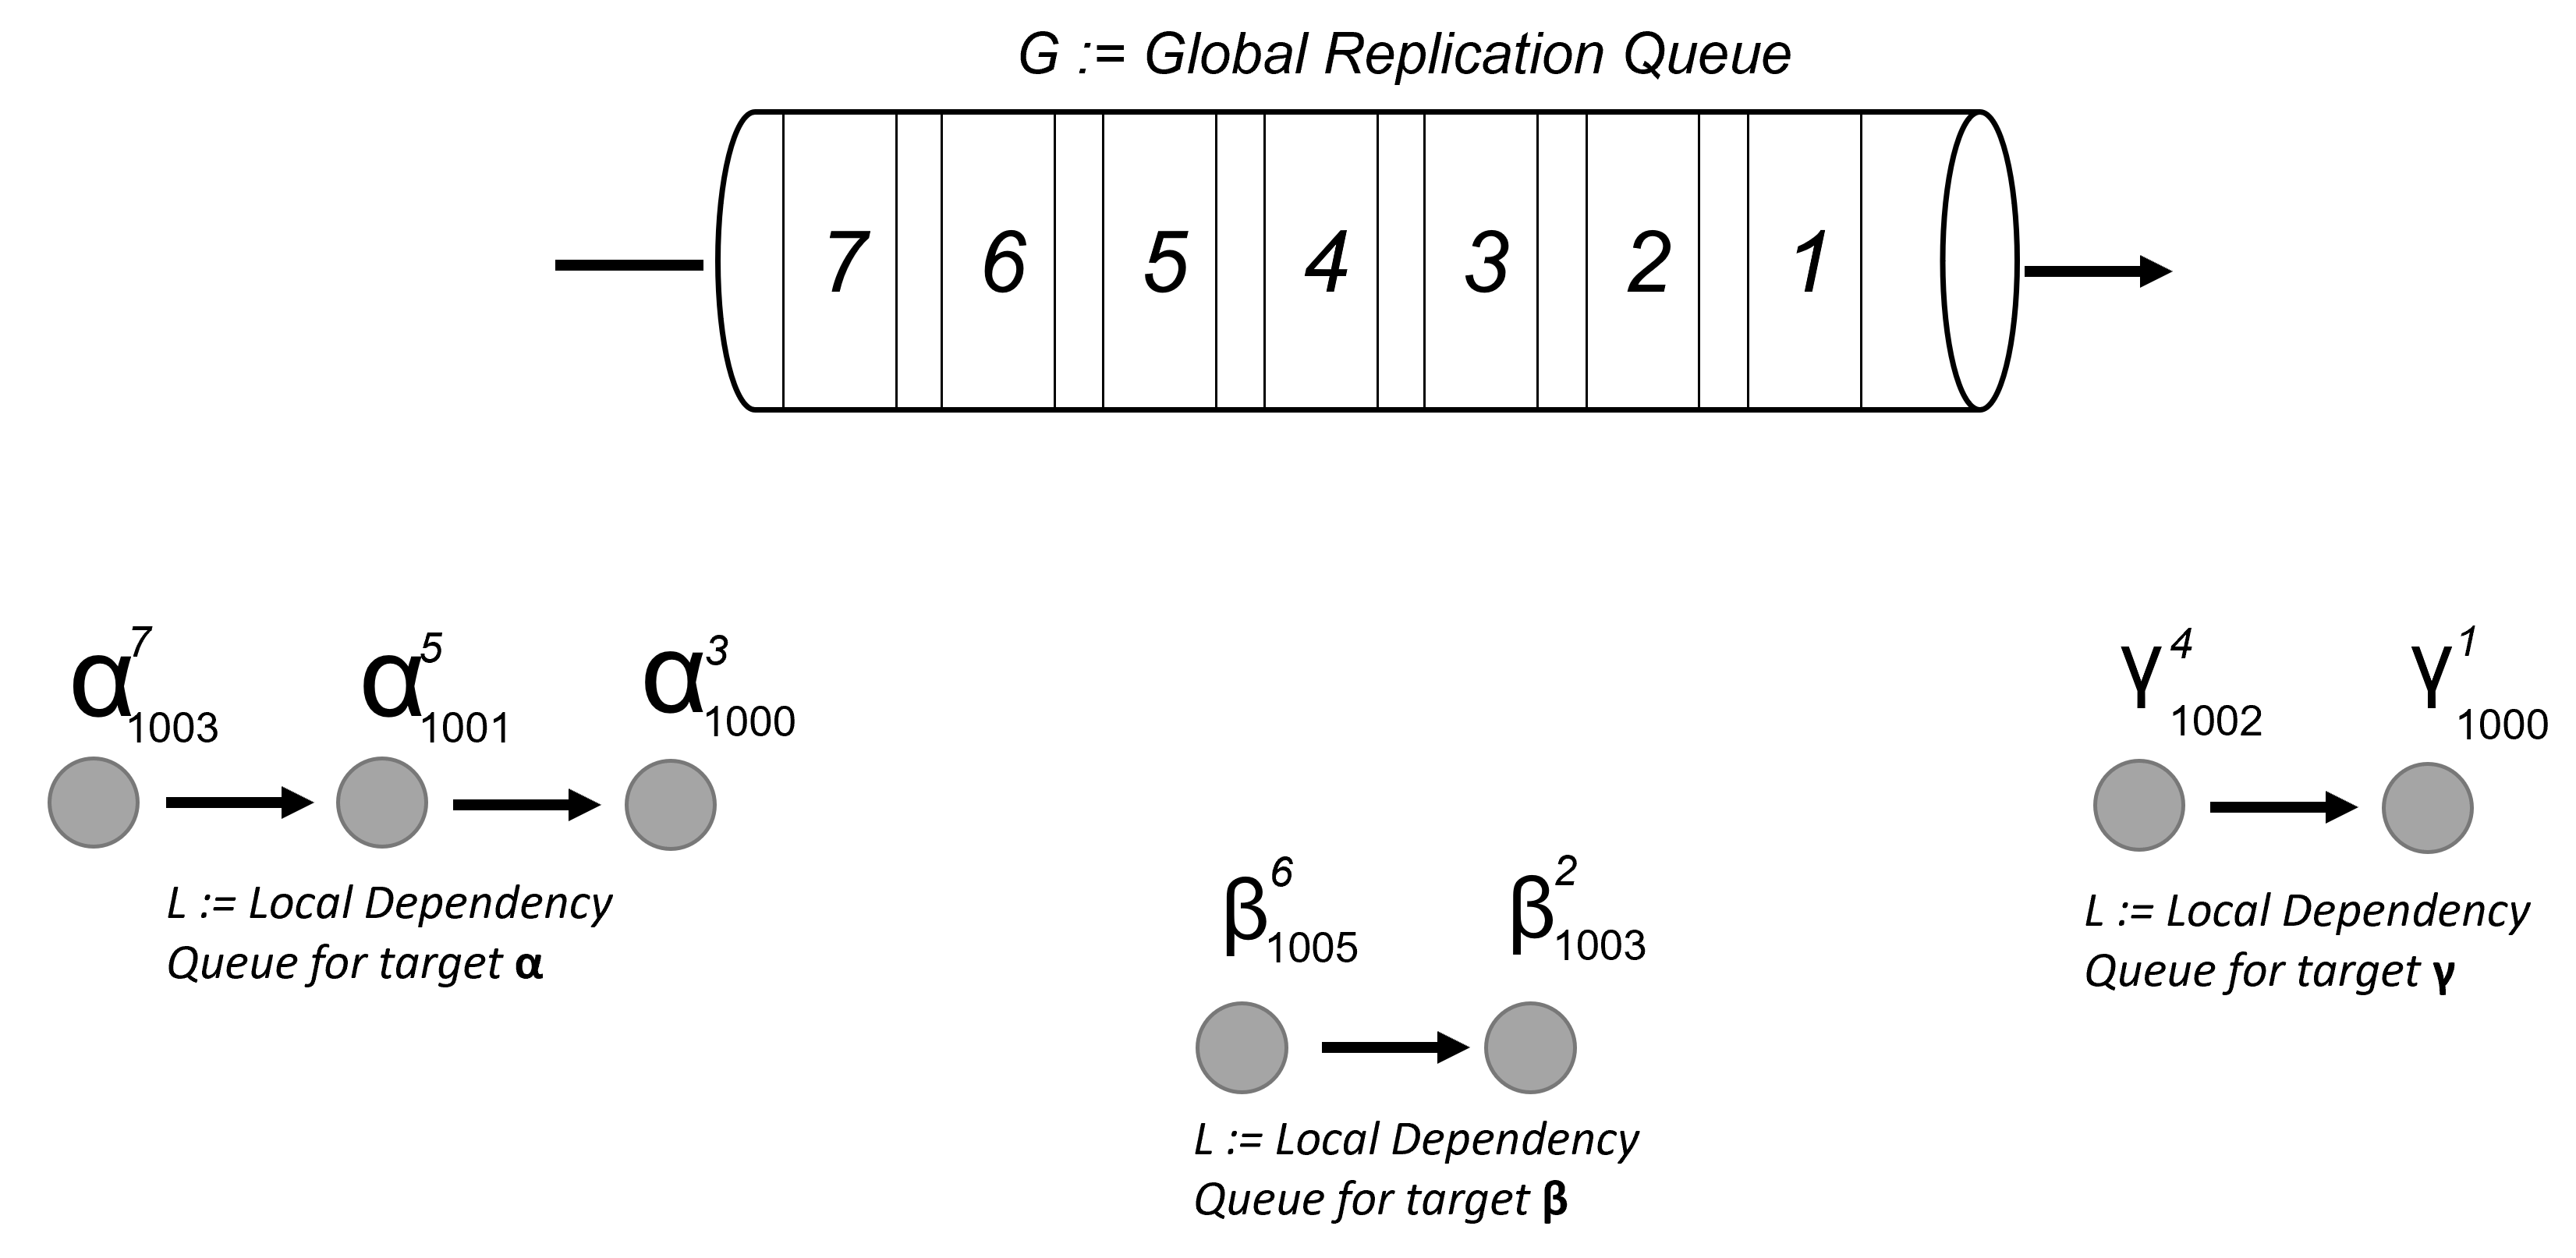
\includegraphics[width=0.8\textwidth]{Figures/Queue.png}
        \caption{Association between global replication queue and local dependency queues.}
        \label{fig:queue}
    \end{figure}
  
    This queue is the core component and the inherent driver revolving around the lazy replication approach. 
    It contains individual replication IDs which correspond to replications targeting exactly one partition placement at a time.
    As depicted in figure \ref{fig:queue} it is represented as a FIFO queue receiving new replication IDs that are registered through the \emph{Change Data Collector} 
    or are rescheduled by \emph{Replication Workers}.\\
    Each replication event within this queue is therefore defined as $x_{z}^y$, where $x$ represents the designated target partition placement, $y$ a global
    replication id uniquely identifiying a specific replication object and $z$ as a reference linking to the actual replication data. 
    Since our replication engine should replicate the data operation-wise, each event within the queue corresponds to one operation associated with one target partition placement.
    Therefore each event can be applied independently.\\Since the primary transaction can only be committed when the data to be replicated has been added to this queue,
    it stores the replication events in-memory to process it faster.

  
    \item[Local Dependency Queue] This queue is defined per partition placement containing pending updates that are yet to be replicated. 
    Since all updates need to be delivered in the same order as they have been applied on the primary replica, they depend on each other. 
    Although labeled and represented as a queue, the entries are saved as an DAG. Where each replication event depends on its predecessor to be executed first.
    Since the entries within this queue are not added concurrently and are ordered according to their execution order, we are certain that the imposed dependency
    reflects the original execution order. If the queue already contains items, new changes will be appended left of the dependency graph. 
    Resulting in the first new item directly depending on the last item currently in the queue, to be executed first. 
    Therefore this queue is used as an utility to enforce constraints on all intermediate steps ensuring that operations are applied 
    in correct order, that all replicas converge equally towards a given target. 


    \item[Replication Worker] These workers are an essential part of the replication engine since they continuously process events from the global queue 
    and initiate the execution. As soon as a worker thread has finished processing a replication, it will take the oldest item from the global queue. 
    Before starting the replication process, it will make sure that this is indeed the next replication to be executed based on the dependency constraints
    within the local dependency queue. If the replication event is not the next to be executed, the worker will re-queue the event, to be proccessed later.
    However, if all prerequisites can be verified a dedicated refresh-transaction is started.
    The one operation is passed on to the \emph{Data Replicator} which will then actually execute the statement on a given target.
    After successful termination, the worker will remove this dependency form the local queue as well as from the replication data. \\
    Based on the current load and the number of pending replications on the system, these workers will be scheduled as needed, allowing to dynamically scale as the system grows.
    Since the \emph{Local Dependecy Queue} always will ensure the correct execution order a concurrent processing of the replicaitons is possible.     
    


    \item[Data Replicator] Is implemented as the actual execution engine which will recreate and execute a captured operation. 
    It is invoked by the replication workers, passing a replication event together with a reference to the corresponding replication data.
    For the Lazy Replication Engine, it will receive one operation per target placement. 
    This has the advanatage that we can now decide based on the targets current placement structure, how to reconstruct the statement. 
    Because this is done right before execution, it shows the benefits of capturing the entire object instead of the statement to be executed per placement. 
    Since this target could have been altered since capturing, it could now have a different set of columns.



    \item[Update Metadata] Since data is essentially stored on physical entities, represented by the internal partition placements, we extended these objects 
    to contain information on general update statistics relevant for this particular placement. These information will be updated at commit time of a write-operation.
    For eagerly replicated placements this is the primary transaction, for lazily replicated however the refresh transaction.
    This enables the system to use this update information to essentially retrieve the current state of the data, represented by the commit timestamp
    and the numer of updates this partition placement has already applied. Allowing us to use those metadata to compare different versions against each other.

\end{description}



With all these services the replication engine is able to process multiple replications at once, while ensuring the correct execution order and stability
for each replication to be executed. 
Since all operations are propagated atomically within one transaction we do not need to worry about a rollback of a refresh transaction or provide complex undo-operations 
to remove those changes. Therefore, these replications can be applied independently per target partition placements and do not interfere with each other, 
allowing for a high flexibility.\\
Furthermore, it does not only replicate the captured modififcations it provides a fault-tolerant approach as well. 
Since Polypheny-DB consists of multiple attached stores that might suffer from outages or local failures, replications might fail.
However since the replication data is centrally stored and is only removed when all dependent replications have been executed, 
a replication event that coninuosuly keeps failing will uneccessarly occupy worker threads and waste storage resources to preserve the data.
Therefore a centrally configured \emph{Fail Count Threshold} is introduced. Everytime a replication fails, the responsbile worker thread will increase the \textit{fail counter} 
of a given replicaiton object. If it reaches the threshold the replication will be removed from the queue entirely. 
Furthermore the traget will be removed from the engine by deleting all remaining local replications for this target as well.
Consequently this particular partition placement will be suspeneded for active data capturing and marked as \emph{INFINITELY OUTDATED}.\\

Due to the architecture of the queue, we can only get an event at the top of the queue. This increases the difficulty to remove all associated replications 
for a target placement at once. However since workers will validate if replications can even be executed and can therefore identify suspended targets, they will
automatically cleanse the queue from unwanted replications, without expensively removing each item within the queue.\\

Moreover contentions can also occur directly within Polypheny-DB, if there are too many pending updates, waiting to be replicated.
Despite the scaling capabilities of the workers the load on the system might still be too high, essentially affecting the main operation on the system.
Therefore we have enriched the configuration to globally enable or disable the replciation distribution. In constrast to labeleing data placements as outdated, 
and removing all pending replications for ever, we can now allow to temporarily stop the replication and only continue to capture modifications. This can help the system
to adapt to high load situations by focusing on its core funcitonality.\\


%%%%%%%%%%%%%%%%%%%%%%%%%%%%%%%%%%%%%%%%%%%

\subsection{Automatic Lazy Replication Algorithm}
\label{sec:algo}

\begin{figure}[t] 
    \centering
    
\includegraphics[width=0.9\textwidth]{Figures/flow_worker.png}
    \caption{Lifecycle of a \textit{Replication Worker} processing pending replications from central queues.}
    \label{fig:flow_worker}
\end{figure}

The goal of the entire lazy replication approach is providing a scalable and fault tolerant approach to distribute the data for each placement onto the designated stores.
Therefore, the algorithm as depicted in figure \ref{fig:flow_worker}, aims to provide a cost-efficient approach to replicate the change data without increasing 
the overhead of the system and impacting regular operations. 
For every DML-operation the routing process will verify which placements need to receive this modification. During this process, all eagerly replicated stores for this entity
are identified. Since all entities contain a list of all data placements, we can compare the delta between the retrieved stores and the actual stores. 
If there is indeed a delta, we can conclude that there are placements which conseqeuntly have to be updated lazily. 
That enabels the entire transaction to \emph{capture change data}. This will directly result in transforming the write-operation of the current statement into a set of basis 
operations, that are already evaluated and can therefore be immediaetely applied to target placements. Consequently a \emph{Change Data Capture Object} will be created, 
containing all information needed to recreate the statement again. Accompanied with the the ID of the current statement as well as the parent transaction this object is prepared
and appended to the capture-queue.\\

During runtime when the statement is about to be pushed-down to the designated stores, the prepared statement is enriched with the pre-evaluated information, 
neccessary to execute the statement. These parameter values are added to the \emph{Change Data Capture Object} as well. 
Accompanied with the parent transaction and the statement id we can identify this change object within the preliminary capture-queue 
and enrich it with the necessary information (see \ref{fig:hashtable}).\\
As soon as the transaction has finished, this object is further processed. If the transaction was aborted and rolledback, we again can directly remove all pre-queued changes 
that are associated with this transaction by removing the entry from the nested hashtable. This will cascadingly remove all attached capture objects.\\
However, if the transaction will be succesfully commited, the finalization phase starts. For all capture objects associated with this transaction the corresponding commit 
timestamp of the transaction will be set. This can later on be used for freshness comparison. Afterwards each capture object will be registered at the \emph{Lazy Replication Engine}. 
To do this, the joint capture object will now be separated into two parts. The first one is the replication data, which contains all information to be applied to 
secondaries as well as all partition placements that shall receive this replication and thus depend on this data. The second one is the creation of independent replication 
objects targeted to individual partition placements. They are bound to a specific operation and responsible for a given target. Additionally they are linked to the single replication data for this change-data set.
This allows us to reduce the data footprint by caching the replication data only once. The list of individual replication events as well as the data is now passed on to the
queue registration. This consequently adds for each target placement a new entry into the global queue. Additonally, it also appends the corresponding replication ID to 
the local queue of each partition placement. Once all replication objects have been added to the global queue the finalization phase ends.\\
Since these capture objects have been added to the prelimiary capture-queue in their execution order, they are also passed on to the actual queue in this exact same order.
This ensures the consistency among the different plaecments, and ensures that they uniformly progress towards a given state as its up-to-date counterpart has.\\

Since this is all still done before the transaction has publicly finished, further operations are blocked until we have asured that all objects have been consequently 
transformed and queued within the associated replication engine. Thus we can ensure the consistency of the secondary placements by waiting until all steps have finished 
successfully. If something would went wrong during queueing, we can still relabel those placments as \emph{INFINITELY OUTDATED}, marking them as not receiving any more updates 
hence informing users and administrators that this placement will stay outdated until manually fixed.\\

After the queing process has finsihed and the primary update transaction has returend, removing all locks, the \emph{Replication Workers} will eventually process the queued events.
As soon as a worker has free resources again, it will take the next item out of the global replication queue and starts analyzing it.
For each item it will verify if this is indeed the next replication to be processed for this target, by obtaining the next item of this partition placements local queue.
Additionally it verifies if the replication distribution has been suspended entirely. This will lead the worker to reschedule the replication
and append it at the end of the global queue again, and moving on to the next item.\\
However if this replication does not exist anymore or this target has been marked as \emph{INFINITELY OUTDATED}, avoiding additional replications to be applied,
the worker automatically cleanses the queue from all remaining replications associated with this placement.\\
Assuming that the currently proccessed event is indeed the next replication in line it will prepare the execution and start a new refresh transaction. 
The data replicator will now analyze the replication event, and ultiamtely reconstruct a new modification statement that will be routed internally towards 
the designated partition placement.
When the replication has finished the item is removed from the local queue. Additonally it removes itself from the dependency graph of the associated replication data.
If the corresponding replication data does not have any dependencies left, it can also be savely removed to reduce the data footprint of the system again and freeing up resources.
However, if the replication process for this target fails, the centrally defined fail count for this specific replication event is increased. 
If it is above the configured threhold, the system will abort further replications of this target placement, labeling it as \emph{INFINITELY OUTDATED} and removing all pending
replications of this replica. Otherwise the replication has been successfully executed.\\

Because the presented lazy update propagation is done operation-wise, we actually loosened the heavy SS2PL constraints that we require on the primary updates. 
Since we already have a serializable schedule after execution, we also know per entity and each partition placement 
the correct execution order that we have to apply the data changes on. So it is not necessary to only free the resources 
after the entire transaction has been replicated but right after each operation. 
However, since Polypheny-DB currently only supports a SS2PL approach we can 
mimic this behaviour by scheduling refresh transactions containing only one modification.
This allows us to replicate data using the less strict 2PL approach, hence improving the overall performance of replications with respect to the primary execution.


%%%%%%%%%%%%%%%%%%%%%%%%%%%%%%%%%%%%%%%%%%%

\subsection{Manual Refresh Operations}
\label{sec:manual_refresh}

Although, the automatic refresh operation, based on the change data capture approach will continuously propagate incoming changes,
it is not able to prioritize certain placements after they have been added to the queue proposed in \ref{sec:lazy:_engine}.
However, users might need to be able to specifically prioritize data placements or entire tables to be updated faster than others. 
This could also be the case if one placement is currently marked as \emph{INFNITELY OUTDATED}.
Either because of too many failed replications or because it was manually configured to remain in a given state. 
As described in \ref{sec:refresh_operations} we need to be able to provide manual refreshes on the basis of primary snapshot copies.
This inherently uses the capabilities of Polyphenys existing \emph{Data Migrator}, which essentially queries a defined source entity on a given store. 
Together with the current \emph{Update Metadata} of this placement, the extracted result of this query can be considered as a snapshot of a given replica.
The contents of this result will be subsequently applied onto a targeted placement.\\
After the data migration process has finished, the target receives its new update information on the basis of previously extracted metadata.
If this placement had remaining replications in its local dependency queue, they are all removed to avoid adding data twice. 
The system then autoamtically switches the replication state of this placement to REFRESHABLE, starting to activiely capture changes again.
Since the snapshot merely depends on the source, only a short-lived shared lock is applied until the data has been extracted. Apart from this, the snapshot will have no impact
on the actual system.\\


Despite that data resides on the partition placmenets, users may only directly interact with a data placement of an entity.
We therefore either allow to manually refresh one specific data placement respectively all partition placements residing on a given store or an entire table.

\begin{lstlisting}[language=sql, caption={SQL Statement Syntax for an On-Demand Refresh Operation},label={lst:refresh}]
ALTER TABLE tableName REFRESH ( ALL PLACEMENTS 
                              | PLACEMENT ON STORE outdated_store );
\end{lstlisting}

Although such refresh-transactions can be executed on any placement, it will have no effect on primaries. 
The same holds for placements that are already up-to-date with respect to their corresponding primary-version, where the execution will be simply omitted.




%%%%%%%%%%%%%%%%%%%%%%%%%%%%%%%%%%%%%%%%%%%

\subsection{Placement Constraints}
\label{sec:constraints}

Since we are in a distributed setup, we always need to ensure that we do not lose any data, while transforming the indidivdual placements. 
This already starts by defining the replicaiton strategy. Although Polypheny-DB allows to customly distribute an entity across several stores, we have to enforce that no 
information is lost. This means that since we can arbitraly place any combination of columns and partitions of a given entity of any store, we need to make sure that at the end, 
each column is represented by all available partitions at least once. Otherwise this would violate the integrity of our system. 
This consequently needs to be considered for outdatedness as well. Since we have decoupled updates of eagerly and lazily replicated placements, we again could lose data. 
Therefore we again have to ensure that at least the eagerly replicated placements are sufficently configured such that each column is available for all partitions at least once.
The remaining secondary placements however can again be arbitrarly combined without any requirements.\\
Because it is possible to switch freely between LAZY and EAGER strategies even after they already contain data, we again have to verify that no data is lost.
Therefore when trying to switch from LAZY to EAGER, we have to ensure that this placement does not contain any pending updates, otherwise the operation will fail.
If there currently are no pending updates the system will lock the entire table, so it will not receive any updates while switching the strategy internally. 
Since this is merely done by setting a flag, the impact of the blocking behaviour can be neglected.\\

Furthermore, as stated in \ref{sec:states} it is possible to switch the replication states of all partition placements of a given data placement from REFRESHABLE to 
INFINITELY OUTDATED and vice versa.
While the manual switch to INFINITELY OUTDATED is an intentional suspension of the replication procedure, the other direction requires validating possible deviations.
If this is not correctly ensured, and the replication starts propagting changes towards this placement again, we will lose data the data in between thos versions.
In this scenario the system first will need to make sure that the placements on this store are all uptodate. If this is not the case the operation will fail. 
This can be also be done manually by executing a \emph{Primary Snapshot Copy} as described in \ref{sec:manual_refresh}. A subsequent change of states will then be accepted.\\

Finally, despite its ability to remain operational during failure situations, the utilzed queues within the engine are still only stored within main memory.
Although this increases the overall commit time of a transaction it results in a loss of all captured data that has not been applied yet, as soon as the system 
shuts down for any reason. Since we rely on the fast registration process to commit the primary transaction as fast as possible we need to mitigate this behaviour.
Since we always know which placments are updates lazily, the replication engine can immediately provide two different mechanisms that can be centrally configured. 
The first approach is simple and fast to execute. It gathers inforamtion on all placements that need to be updated lazily. It can automatically mark them as INFINITELY OUTDATED, 
and therefore suspending any more replications. Users can either choose to update the system manually or refreshing is on read as proposed in \ref{sec:refresh_strategies}.
The second approach however results in a much slower startup time by refreshing all placements first, before the system will even start.




%%%%%%%%%%%%%%%%%%%%%%%%%%%%%%%%%%%%%%%%%%%%%%%%%%%%%%%%%%%%%%%%%%
%%%%%%%%%%%%%%%%%%%%%%%%%%%%%%%%%%%%%%%%%%%%%%%%%%%%%%%%%%%%%%%%%%
%%%%%%%%%%%%%%%%%%%%%%%%%%%%%%%%%%%%%%%%%%%%%%%%%%%%%%%%%%%%%%%%%%





\section{Freshness Awareness}

With the Lazy Replication and the accompanied defferal of transactions prepared, we have already established a foundation to use those possibly outdated versions
for freshness-awareness.

This section therefore focusses on all aspects to establish the core aspects of freshness within Polypheny-DB,
to allow users the specification of freshness and efificiently using those outdated placements to distribute the workload across the system.
The actual freshness evaluation can therefore be separated into roughly two phases. While the first one uses the specified freshness tolerance to generate an 
applicable filter to identify suitable candidates. Whereas the second phase is concerned with constructing and selecting possible combinations of outdated versions
to provide an efficient workflow.


%%%%%%%%%%%%%%%%%%%%%%%%%%%%%%%%%%%%%%%%%%%

\subsection{Evaluation Types}
\label{sec:eval_types}

As delivered through the concept in section \ref{sec:freshne_metrics}, there exist several possible freshness metrics to use for version comparison.
These metrics are primarly used to filter placement candidates based on a defined freshness based on their \emph{Update Metadata}.
We have summarized these possibilities and established three different evaluation types, that can be used to specify an accepted level of freshness.


\begin{description}
    \item[Timestamp] A timestamp is the most simple form of a freshness evaluation type, since it intuitively provides the capability to define 
    an acceptable lower bound of outdatedness, for a specific query. Potential partition placements are therefore filtered by verifying that there commit timestamp is newer
    than the specfied one. Otherwise they are removed from the list of possible candidates.
    
    \item[Time Delay]
    The time delay can be specified together with a time and an associated time unit to define an accetable delay for the desired freshness. 
    This will intuitively substract the specified \emph{Absolute Time Delay} from the current time generating a lower bound timestamp. 
    This again allows filtering all partition placements based on the age of their commit timestamp.
    Again as described in \ref{sec:freshne_metrics}, an absolute time delay based on the current time is not always accurate or might even render wrong results.
    Therefore, a \emph{Relative Time Delay} specification is provided as well. Allowing to specify the tolerated time deviation based on the commit of a primary placement 
    compared to an outdated placement. To differentiate those options they are individually suffixed with either \emph{ABSOLUTE} or  \emph{RELATIVE}.

    \item[Freshness Index]
    Naturally it expresses the freshness specification based on the modification deviation between an up-to-date placement
    and a refreshable placement. The \emph{Modification Deviation} therefore allows comparing the number of modifications of specific partition placements
    to define a freshness index. For a query this index can be either configured to filter based on each partitions placements deviation or on their accumulated deviation.
    Therefore the number of modifications is accumulated and then compared against the accumultaed number of modifications 
    of all up-to-date entities that have been considered within this query. This allows a more stable approach since it is not prone against outliers. 
    Furthermore, this index can also be configured using the freshness index to evaluate the \emph{Time Deviation} between two replicas. 
    Essentially the index dictates how accurate a given placement is with respect to its up-to-date replica.
    
\end{description}

Since these evaluation types are fundamentally different in terms of version comparison, they
allow users to indicate their tolerated level of freshness, depending on their requirements or preference. 


%%%%%%%%%%%%%%%%%%%%%%%%%%%%%%%%%%%%%%%%%%%

\subsection{Query Specification}
\label{sec:fresh_spec}

Equipped with the evaluation types, users now need to be able to define their intended level of freshness.
Although that this could be centrally defined for an entire system, it is very subjective and often does not even depend on the user
but is rather influenced by application-specific requirements.
Therefore, the specification should be rather defined on a query level, to allow a more fine-grained definition.\\

This can be achieved by extending the query functionality of Polypheny-DB, allowing users to directly specify their demands.
Although Polypheny-DB provides multiple query interfaces and languages, the following specifications are solely demonstrated with SQL. 
As proposed within section \ref{sec:eval_types} we have introduced three freshness types that can be used to specify a tolerated level of freshness.
These support all freshness metrics as described in the corresponding section \ref{sec:freshne_metrics}. Along the functional 
requirement \textit{(ii)} all these metrics have been introduced within Polypheny-DB.

For SQL, the query syntax is extended  with an optional leaf expression at the end of every query to generally support freshness specifications. 
Along the description, users can choose to select any of the presented evaluation types to guide the system if and how it should consider the freshness of an entity.
\begin{lstlisting}[language=sql, caption={Generalized Freshness Specification},label={lst:general}]
SELECT * FROM tableName [ WITH FRESHNESS [ <TIMESTAMP> | <DELAY> | <INDEX> ] ];
\end{lstlisting}

The statement depicted in \ref{lst:general} illustrates a generalized and abstracted freshness specification including placeholders for the different evaluation types.

While a statement with an explicit evaluation type provides a direct intent, users can also choose to solely specify \emph{WITH FRESHNESS} 
and omit the type, to implicitly suggest that you will consider all outdated data regardless of the actual version.





%%%%%%%%%%%%%%%%%%%%%%%%%%%%%%%%%%%%%%%%%%%

\subsection{Freshness Processing}
\label{sec:fresh_proc}

As for every query, a freshness-statement is first transformed into a tree, parsed and evaluated in terms of syntactical correctness. 
Additionally, the query is analyzed semantically where also the specified freshness will be extracted. The designated \textit{Freshness Extractor} 
validates, if the provided freshness evaluation type even exists and if the specified values can even be associated with this type.
Furthermore it verifies if the specified level is in bound of the possible value spectrum. 
Otherwise the statement cannot be executed and will be canceled.\\
If the query and the freshness specification have been successfully analzyed the extractor generates a designated \textit{Freshness Object}, 
containing all specified freshness details. This will be attached to the statement to be used for further processing.
It automatically helps to enrich the statement with the correct freshness information and informs the transaction that freshness is being used,
which directly influences locking capabilities and changes the routing process. 
Along with requirement \textit{(vi)} as stated in \ref{sec:tx_handling}, this will transform the transaction to read-only mode, prohibiting the execution of any more DML
statements. This is necessary to avoid that a write-operation uses outdated data retrieved within this transaction to update a placement.\\

Since freshness-awareness allows to read data that is considered to be stale, we implicitly support \emph{Dirty Reads}, hence violating the ACID properties.
Therefore the read-only transaction now allows to omit locking entirely, by enabling the new isolation mode \emph{None}. 
Compared to the conventonal isolation mode \emph{Serializable} which enforces locks on the basis of SS2PL to provide correct concurrency control, \emph{None} 
loosens all constraints. This causes refresh operations to override or add new results to the entity while it is currently being read. 
Beside the obvious benefits of allowing more parallel load on the system, it has a positive effect on the replication as well.
Since the provided CDC approach is designed to continuously provide the placements with captured updates, the target placements will be almost consistently locked due 
to the number of write-operations.
With a \emph{Serializable} isolation level those replicas could not be used for freshness related queries after all. 
This would completely mitigate the performance gained by decoupling the transactions in the first place. 
Therefore, if not centrally configured or explicitly specified otherwise, every freshness query will natively omit the lock acquisition to provide even more parallel workload.\\


%While this is not heavily impacted by consecutive write-operations that are lazily replicated onto this placement, it could return entirely inconsistent data when 
%an placement is being refreshed through the Data Migrator. 
%Because such manual refresh operations will comprehensively transform any entity and placement it requires to set a \emph{Refresh-Lock} even for outdated placements 
%until the data migration has finished.
%Although not technically considered to be equal with a \emph{Shared-} or \emph{Exclusive-Lock}, it will flag this placement as not available for queries anymore and therefore will
%refrain from allowing anymore locks to be added.\\


Although, not neccessary for all queries, users still might desire to read outdated data without having to fear that the data will be refreshed while reading.
Since Polypheny-DB essentially uses 2PL, shared locks can be easily extended with more transactions adding themself to the list of already waiting transactions.
Despite that this avoids \emph{Dirty Reads} and the results will stay stable and consistent, it will block further refresh operations on this placement entirely. 

This however could then lead to starvation of the refresh transactions. 
Therefore we embedded an extension to this locking approach especially for this use case, which does not interefere with 
the locking mechanism that targets primary copies. When there is currently a shared lock on an object that is about to receive a manual refresh operation, 
this disables the possibility for any new upcoming freshness transactions to add itself to the existing shared lock. Instead they are treated and added to the dependency graph 
of the refresh operation an its Refresh-Lock, as if there would already be an exclusive lock in place. 
This would avoid starving the refresh operation while still being able to serve freshness queries on different placements.
This can be further enhanced by centrally configuring \todoMissing{implement} a threshold, which defines after how many retries the refresh operation can finally force itself 
to be executed.\\
While the previous approaches simply tried to provide any possible combination
and construct a result out of different independent versions, the last charcteristic goes a step further and allows to specify a referential integrity enforcement. 
As described in section \ref{sec:read_access} this approach aims to enforce the referential intergity among all entities used within the transaction, 
allowing to retrieve a cross-entity result that was valid in the past. Since it builds on top of the previous characteristic is also needs to lock the placements. 
However in our implemented scenario, other than in classical multi-version databases, we are not even guaranteed that every entity even has several versions. 
Therfore we require for such a query that all relevant placements need to be updated by the same original transaction in order to guarantee that this state is valid.
However if there is doubt or no suitable combination of placements can fulfil this request,
we always have the possibility to fallback to the primary nodes, which are guaranteed to support referential integrity.
Allthough, this again will again block updates on the primary placements, it fulfils the constraints as it would have, when executing the same query without specifying a tolerated level of freshness.





%%%%%%%%%%%%%%%%%%%%%%%%%%%%%%%%%%%%%%%%%%%

\subsection{Freshness Filtering}
\label{sec:fresh_filter} 

\begin{figure}[t] 
    \centering 
    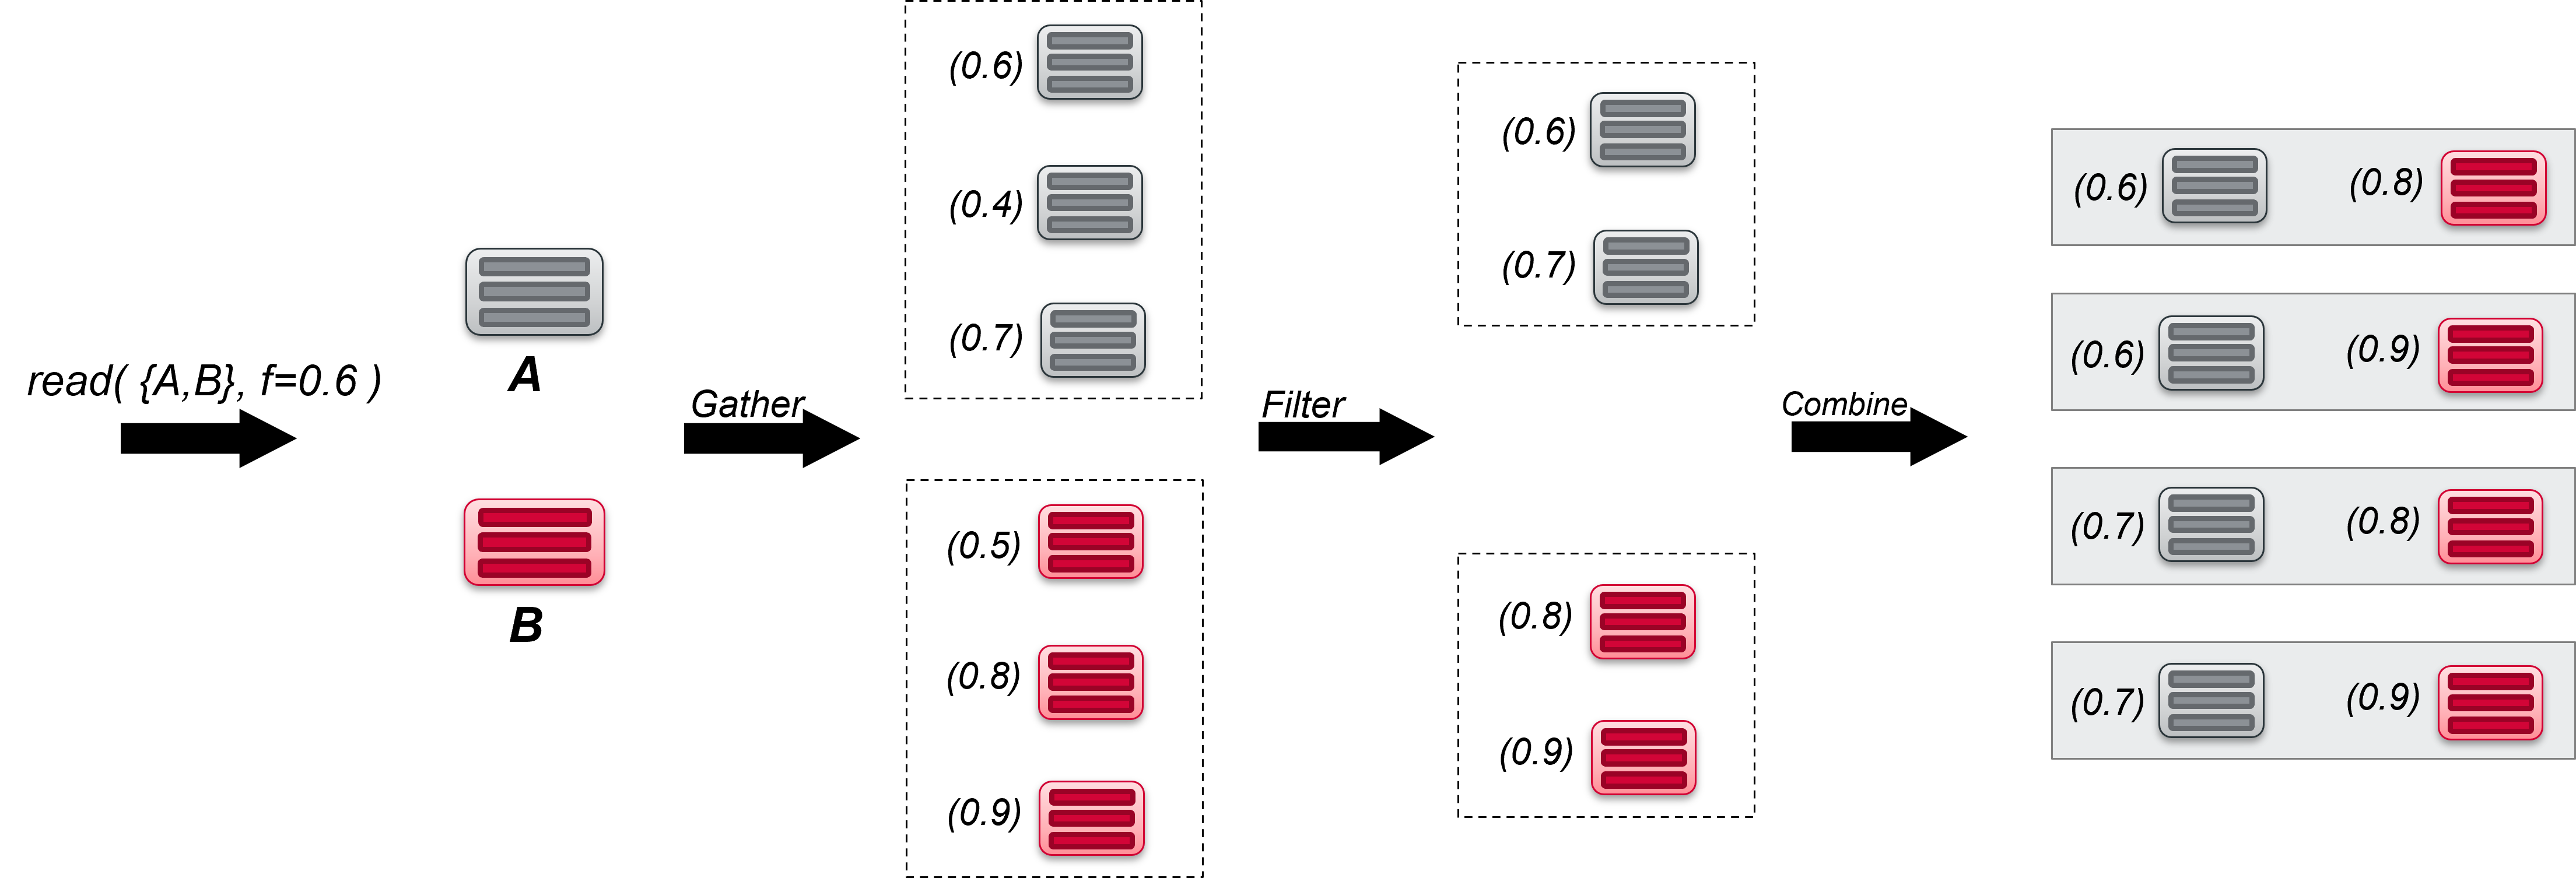
\includegraphics[width=0.9\textwidth]{Figures/filter.png}
    \caption{Subsequent Filter Operations for an abstracted freshness read operation, generating several possible execution plans based on a given freshness-index.}
    \label{fig:filter}
\end{figure}

The \emph{Freshness Manager} is the heart of the freshness evaluation and will consequently assist the routing and selection process to propose eligible placements
to be used for retrieval. 
It aims to apply and analyze the freshness specification captured within the \emph{Freshness Object} of a given statement and transform it 
into a general filter condition (\emph{Freshness Filtering}). These filters will be directly derived from one of the selected evaluation types described in \ref{sec:eval_types}.
Initially the routing process will first assess which partitions of the requested entities are needed to provide a result.
This is an independent step and will be done regardless, whether a regular or a freshness query ist processed. 
A list of all required partitions is then passed on to the Freshness Manager, along with the associated Freshness Object. 
As already described above, we have applied our versioning on the basis of partition placements, since they represent the actual physical tables,
the freshness filtering and evaluation is therefore always executed by comparing the \emph{Update Metadata} of individual partition placements. 
Disregarding the actual type, the Manager then retrieves all partition placements for each required partition that are considered to be updated lazily.
Aforementioned this can be easily retrieved since these are represented by the Replication Strategy: \emph{LAZY}, which is configured within each placement. 
This operation will consequently generate a data-structure, mapping the required partitions to a list of potential partition placement candidates.\\

With these candidates the type-specific filter function is invoked. Each evaluation type and freshness specification has its own filter functionality and
processes the placements differently. This is mainly done using metadata within the update information properties of each partition placement. 
These already contain information on the current commit and update timestamp,
the original parent transaction which has updated this placement as well as the number of modifications this particular placement has received.
These information can be consequently used to compare their state against the corresponding primary placement with the same partition. 
While \emph{TIMESTAMP} and \emph{DELAY} can be used directly to assess the cadidates, the utilization of an \emph{INDEX} needs an intermediate computing step.
Disregarding the delay being based on modification- or time-deviation we have to calculate per potential placement its designated index.
Naively the filtering can then be done by ensuring that placments are only kept among the candidates if they fullfil the constraint and are above 
a given tolerated threshold. However, for the deviation types we also allow to assess the freshness jointly among all possible candidate combinations.
This means instead of filtering on the basis of single candidates we extend this notion to be able to filter based on their acccumulated freshness when combining the placements
(see \ref{sec:fresh_select}).
Since our query can require multiple partitions at once, we could now combine a very fresh placement with a placement that is by itself considered to be too outdated.
While the individual placements might not fulfil the placement, their combination migth do. Allowing to consider more candidates, hence tolerating outliers.
Due to the possible strong fragementation of versions with this approach, it is not used by default and needs to be configured separately.
Based on the final filter application or already on the intial pre-mapping of partitions we can resepctiviely identify if we have sufficiently collected partition placements 
for all partitions. If one map should be empty, the freshness manager will halt and automatically fallback to a regular routing appoach, targeting only primary placments 
as if freshness has never been specified. \\
Although theoretically an empty partition mapping would not require the entire processing to fallback to the primary version, and 
would be able to solely provide a primary copy for this partition alone and still allowing to construct the freshness, 
for the remaining partitions. 
However, we need the system to provide a seamless and reproducible approach for users, and strictly distinguish between regular and freshness operations. 
Additioanlly as defined with requirement \textit{(vi)} we should not interfere with the primary versions of the system, resulting in a defined fallback scenario whenever the freshness
criteria cannot be uniquely fulfilled.



%%%%%%%%%%%%%%%%%%%%%%%%%%%%%%%%%%%%%%%%%%%


\subsection{Freshness Selection}
\label{sec:fresh_select}

The combination of possible candidates is also executed within the \emph{Freshness Manager} and builds on top of the candidates proposed by the \emph{Freshness Filter}.
It tries to combine accepted candidates with each other, in order to provide possible executable plans, as visualized in figure \ref{fig:filter}.
While this step is trivial if we only have one possible candidate per partition, it becomes more complicated for entities containing multiple placements 
with several partitions. This could easily result in large permutations and possibilities to combine the different placements with each other.
Therefore, selecting a suitable combination is often time consuming and can lead to performance impacts, 
resulting in freshness queries to be less efficient than regular queries due to the enlarged processing times. 
But, since the introduction of a freshness notion is inherently driven by the pursuit to reduce locking and speed up queries we have to 
retain additional overhead as much as possible. 
While the first steps during filtering need to be applied for every freshness-query, the combination step should therefore be executed as little as possible.

As discussed in Polypheny-DBs architecture (\ref{sec:routing}), the routing is essentially decoupled into four parts.
Whereas the \emph{planning part} is the most complicated one, since it also needs to generate potential plans which can later be used during the selection phase 
to be executed. Because this is very time consuming it allows to utilize pre-cached plans to skip this expensive phase.
Therefore our freshness combination process should be attached to this phase as well. \\

If based on the filtered placements the \emph{Freshness Manager} now recognizes that there are too many possible combinations, and the planning would 
exceed a common processing time, the actual planning and combination phase is deferred to be executed asynchronously.
However a suitable substitute plan needs to be provided to still fulfil the request.
While it is always save to simply return the result generated by a primary execution plan, we can also choose to simply select one of the generated candidate plans, before
the \emph{Freshness Manager} has decided that this computation is too expenssive and will be deferred. 
The deferred planning phase can then be executed at a later point in time, to decouple the time-consuming combination of candidate placements from the actual execution.
These generated plans associated with a given query can then still be added to the cache, to be reused next time.
If during processing we then indeed can involve cached plans for a similar query, the planning can be omitted.\\

The selection of these cached plans and their encompassed placement combinations then ultimately depends on indivudally specified attributes.
These could be allowing dirty reads, ergo allow refresh operations to be executed during active reads on outdated nodes or if we rather need a soft 
locking approach here as well. This would forbid reading from placements that are currently being updated or forbid updating placements that are currently being read.
However this again reduces concurrent writes and reads on the store imposing possible downtimes and reducing the availability trait.

Since the Freshness Manager always identifies the given freshness first and gathers all possible placement distribution possibilities for a given freshness specififcation, 
we can validate if we have already cached a similiar query where we had the same placement distribution as input. 
This allows us to use the cache, skip the planning phase and avoid generating possible combinations again, to again provide access to outdated data . 

This ultiamtely enables freshness-awarenss within Polypheny-DB to evaluate and utilize the freshness specififcation, to improve the inherently distributed system 
architecture to decouple transactions and efficiently distribute workload to utilize outdates replicas and consequently increase the performance of the entire system.



%Once a given plan has been selected and therefore a specific freshness option has been chosen we will add this information within our transaction.
%Although not necessary for all queries 
%\todoMissing{define that if a given selection was indeed fulfilled within the system, that is should be also configured within the transaction to define again another lowest 
%bound, to allow newer operations within this transaction to only need as new data as possible. Therefore the selection process inherently is derived of using a cost based approach
%by selecting the best canidates in terms of their response time or simply the oldest to have more permutations left when always selecting the oldest.}



